\section{Object Oriented Design}
    Object orientated programming is a very powerful concept but does not always lead to quality
    software. There are 5 principles that focus on dependency management to avoid code that
    is breakable, fragile and hard to maintain. This is why the SOLID \cite{Hotop2015} 
    principles of OOP should be applied.
    SOLID stands for :
    \begin{enumerate}
        \item 
            \textbf{S}ingle Responsibility Principle
        \item 
            \textbf{O}pen Closed Principle
        \item 
            \textbf{L}iskov Substitution Principle
        \item 
            \textbf{I}nterface Segregation Principle
        \item 
            \textbf{D}ependency Inversion Principle
    \end{enumerate}
    In the section below, describes in detail how the SOLID principles are 
    being applied to the navigation module. 

    \subsection{Single Responsibility Principle}
    
    This principle states that there every class should have a single responsibility
    and there should never be more than one reason to change the class. To
    follow the principle a proper division of the modules is required. 
    I decided to break down the code base into 8 packages where each 
    individual modules will go and they are as follows:
    \newpage
    \textbf{Project Package description}
    \begin{enumerate}
        \item 
            \textbf{constants} 
                This package contains constants like the Raspberry pi I/O pin 
                numbers, API endpoints. All the variable which will not 
                change and could be used in the project are normally kept here.
        \item 
            \textbf{presenters} 
                This package contains the presenters for the model and the view.
                The class Navigation Manager is here which is responsible to communicate
                with the view and all the three services (I/O service, GPS service and 
                Direction API Service).  
        \item 
            \textbf{customExceptions}
                This package would contain custom exceptions if created.
        \item 
            \textbf{Interfaces}
                This package contains all the Interfaces for the corresponding classes. 
        \item 
            \textbf{Listeners}
                This package contains custom asynchronous android listeners which gets 
                called when the task get done. For example a listener also known as the
                observer pattern \cite{Hotop2015} to get the result
                from the google API server is also here. It is the most common way of
                making asynchronous calls in android. 
                \href{https://guides.codepath.com/android/Creating-Custom-Listeners}
                {Android custom listener}
        \item 
            \textbf{models}
            This package contains the data layers mainly 
            \href{https://spring.io/understanding/POJO}  {POJO}. Classes defining how the
            data should look like.
        \item 
            \textbf{services} 
                This packages consist of sub packages for the I/O, GPS and Direction service.
        \item 
            \textbf{utils}
                This package has the utilities for making the API requests and other utilities. 
    \end{enumerate}

    \par
        \label{ssec:srp}
        Figure \ref{fig:directionServiceClassDiagram} presents the class diagram
        of the Direction API services. This is the main task that is explained
        in the chapter \ref{sec:introProblemStatement}.
        The package Direction Service API is further divided 
        into more packages i.e. Google Direction API service. This package 
        structure is maintained to achieve cohesiveness \cite{AdamCarlson}. Cohesion
        is a way to measure how much a segment in a code belong together. 
        
        \par
        The Google Direction API service contains the actual implementation 
        which make requests to the server and fetches back the result to the 
        presenter \cite{mvp} for further processing. This package is also split up into 
        two concrete implemented class and a abstract interface. The reason
        for splitting them in the manner is again the same to preserve cohesion
        and decoupling which is stated by the Single responsibility principle.
        The classes are explained more in detail in the list below. 
        \begin{enumerate}
            \item 
            \textbf{GoogleDirectionAPIService}
                This class is main class which is exposed to the presenter. It is
                responsible to give the input parameters to the Google direction 
                middleware, run the request in a thread so that the program is not
                blocked using \href{https://developer.android.com/reference/android/os/AsyncTask.html}
                {Async Task Util} this can be found in the util package and the using a listener
                retrieve the results back after the completion of the asynchronous call.
            \item 
            \textbf{GoogleDirectionAPIMiddleware}
                As the name states it this class is a middleware where the instantiation
                of the HTTP client framework \href{http://square.github.io/retrofit/} 
                {Retrofit} and configuration is being done. It is responsible
                to interface between the google API server and the client.
                This class is separated to ensure cohesiveness and decoupling.
            \item 
            \textbf{IGoogleDirectionApiService}
                This is an interface for the Retrofit framework which defines the input
                parameter to carry out the HTTP request to the server.
        \end{enumerate} 

        % Write about why I decided about the two classes and how single responsibility is behind this decision  \ref{fig:directionServiceClassDiagram} 
    \begin{figure}[htbp!]
        \centering 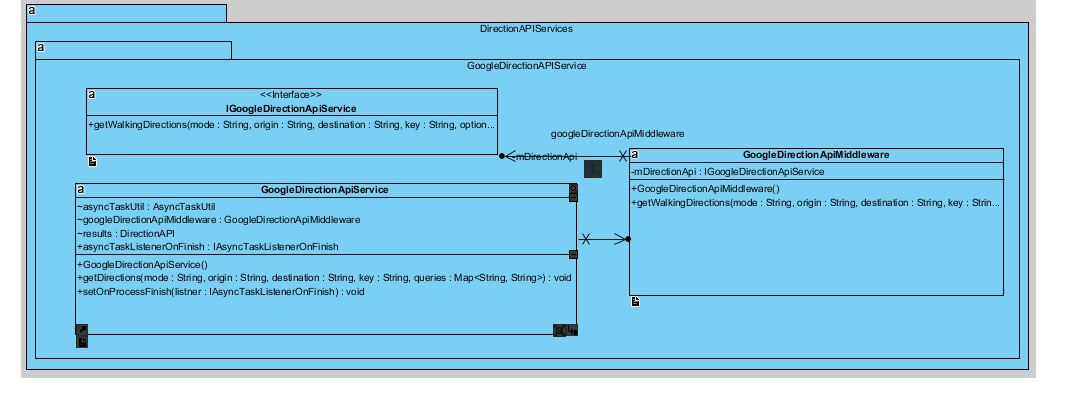
\includegraphics[scale=0.6]{grafiken/directionService.jpg}
        \caption{Class Diagram: Design of the Direction API service}
        \label{fig:directionServiceClassDiagram}
    \end{figure}
    \subsection{Liskovs Substitution Principle}
    Liskov Substitution Principle states the following: " If for each object A of type S
    there is an object B of type T such that for all programs P defined in terms of T,
    the behavior of P is unchanged when A is substituted for B then S is a subtype of T"  
    \cite{Hotop2015}. This principle is taken into careful consideration for design 
    because it gives us the flexibility to replace the implementation in the dependent 
    class without modifying the other objects coupled to it. 
    \par
        Following figure \ref{fig:navigationManagerClassDiagram} the attributes declared
        in this class are i.e. IDirectionApi, IGPSservice (the I prefix in a notation is for
        an interface) which are just abstractions instead of the concrete classes.
        Designing it in this way it would be possible to replace GoogleDirectionAPI service
        with any other realization and the Navigation manager would not see the difference.
        The only criteria is the concrete implementation should implement the interface
        which is exposed. An Example can be seen in the code \ref{code:liskovExample}

        \newpage
        \begin{lstlisting}[
            caption={Example of Liskovs susbstitution},
            label={code:liskovExample},
            language=java
            ]
            public class GoogleDirectionApiService implements IDirectionApi{}

            public interface IDirectionApi {
                void getDirections(final String mode, 
                    final String origin, final String destination, 
                    final String key, 
                    final Map<String,String> queries);
                void setOnProcessFinish(IAsyncTaskListenerOnFinish listner);
            }

            public class NavigationManger  implements INavigationManager {
             IDirectionApi googleDirectionApiService
            }
             
        \end{lstlisting} 

    \begin{figure}[htbp!]
        \centering 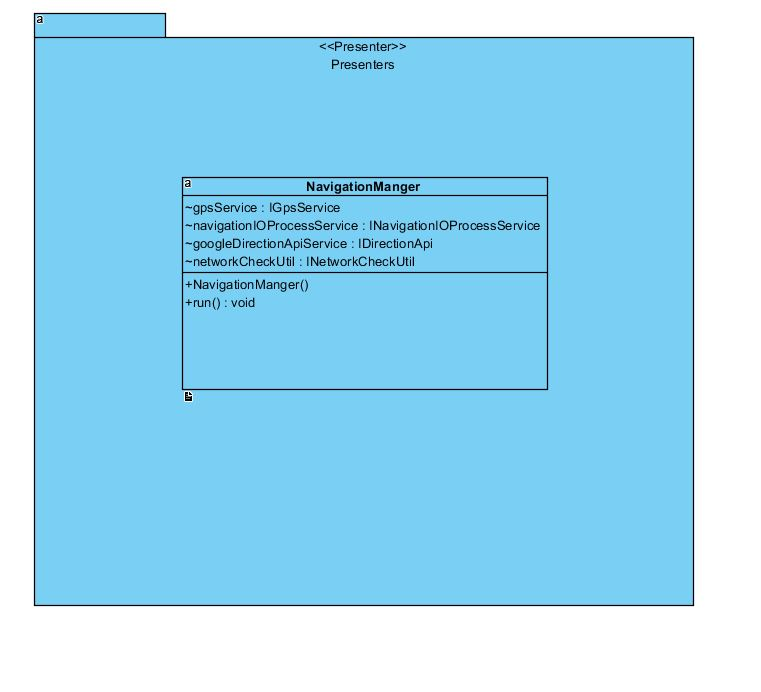
\includegraphics[scale=0.6]{grafiken/liskov.jpg}
        \caption{Class Diagram: Design of the NavigationManager}
        \label{fig:navigationManagerClassDiagram}
    \end{figure}
    \subsection{Dependency Inversion Principle}
    This principle states that higher level modules should not depend on 
    the low-level modules but they should both depend on abstractions. If one class 
    knows explicitly about the design and implementation of another class,
    the change made to one class could break the other classes. This could
    create a series of rippling effects to break the program and DI can help avoid this. Figure
    \ref{fig:DIExample} gives us an overview of the principle.

    \begin{figure}[htbp!]
        \centering \includegraphics[scale=0.85]{grafiken/di.jpg}
        \caption{Dependency Inversion example
        \href{https://upload.wikimedia.org/wikipedia/commons/9/96/Dependency_inversion.png}{ImageRef}}
        \label{fig:DIExample}
    \end{figure}

    \par
        Dependency Inversion will be achieved in this module with the help of a dependency
        injector \href{http://square.github.io/dagger/}{Dagger} 
        \ref{appendix:dagger}, 
        which 
        will be used to inject the dependencies into the classes. 
        This framework is responsible for creating and managing the 
        objects and injecting them to the required
        class. 
        Figure \ref{fig:DIComparision} shows a snippet of a class 
        NavigationManager one without DI and one with DI.
        It can be seen that in the code which is not using 
        DI the dependencies are tightly coupled because all the
        dependencies are handled inside the class NavigationManager.
        Using DI the object creation is being handled by the
        framework which would lead to decoupling of these dependencies.

    
        